\setlength{\footskip}{8mm}
\chapter{ Experiments and Results } \label{experiment}
This chapter describes the results of the road lane detection and lateral 
distance estimation of the car to the lanes.

The video was recorded at 30 frames/seconds using a digital camera (Fuji FinePix 
S9600) which was attached to the camera tripod and placed it in front of the passenger seat as shown in Figure 
\ref{fig:camera_in_car}. 

I implemented the program using standard C++ running on a normal commodity 
laptop. 

\begin{figure}
\centering
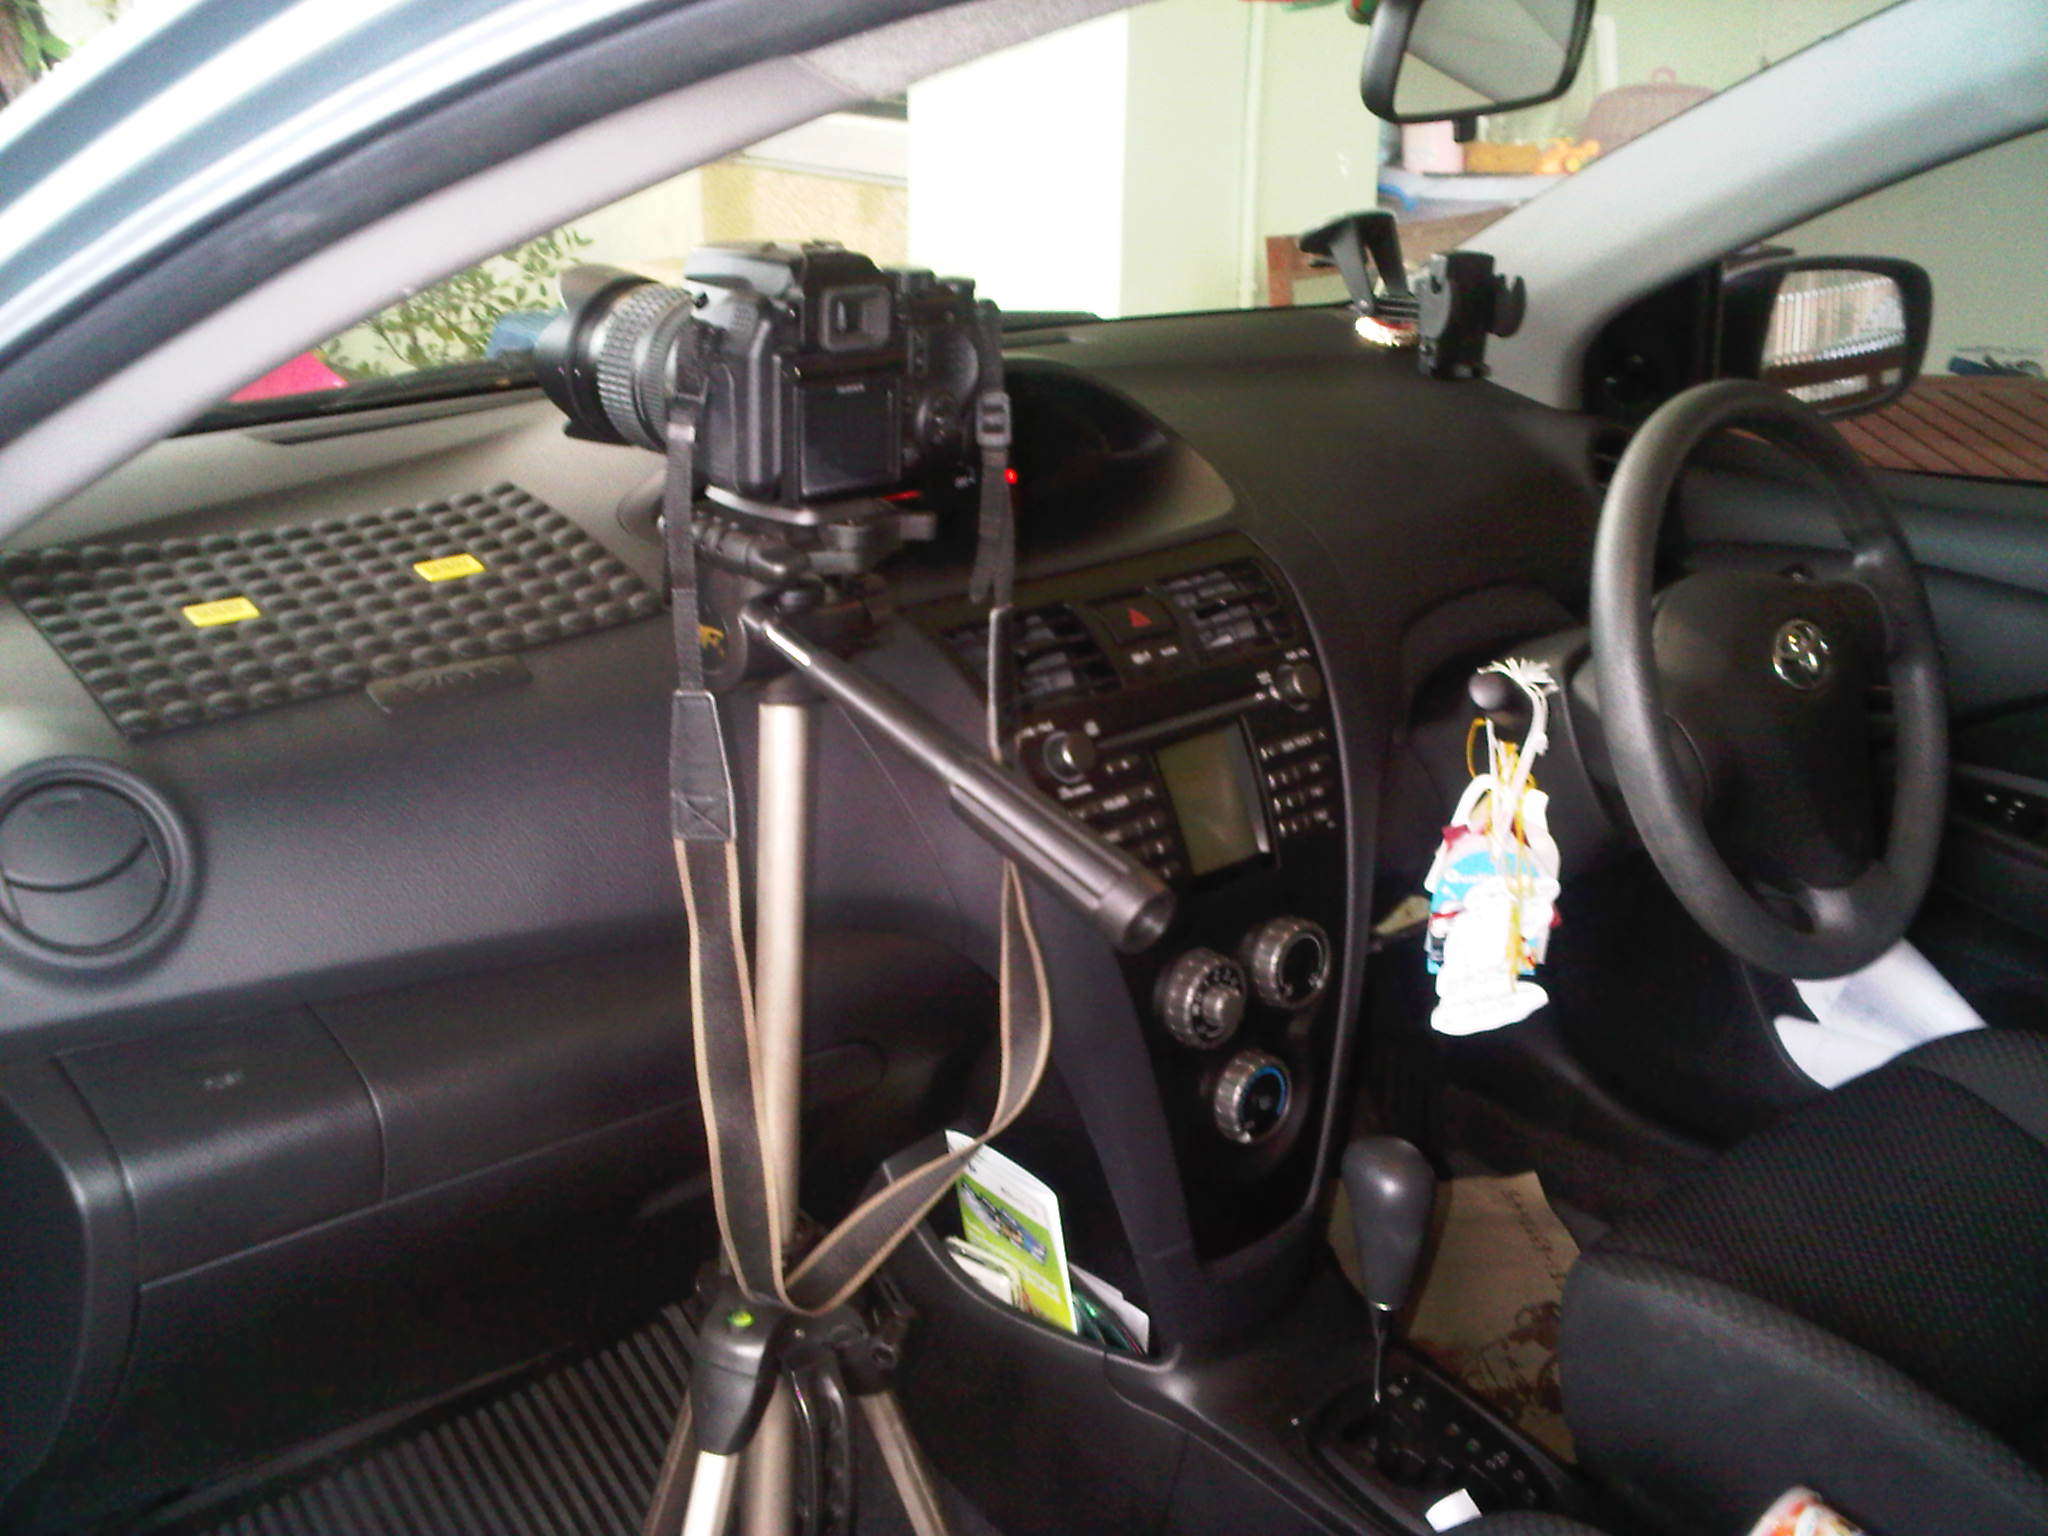
\includegraphics[width=100mm]{figures/camera_in_car.jpg}
\caption{The camera is placed in front of the passenger seat to record the video. }
\label{fig:camera_in_car}
\end{figure}

\section{Matched Filter Convolution}
Figure \ref{fig:matched_filter_convolution} shows the results of performing the 
``Matched Filter Convolution" on the input image. The figure from left to right 
are the input image, the results of matched filter convolution and non-maximum 
suppression. 

Figure \ref{fig:matched_filter_convolution}(a) shows the results of an input 
where the road lane is clear and there is no object near by. Figure \ref{fig:matched_filter_convolution}(b) shows the results where they are white stripes in the middle of the lane. Figure \ref{fig:matched_filter_convolution}(c) shows the results of a long lane markings and dashed lane marking. 

\begin{figure}
  \begin{tabular}{c c c}
    \includegraphics[width=55mm]{figures/original1.jpg} &
    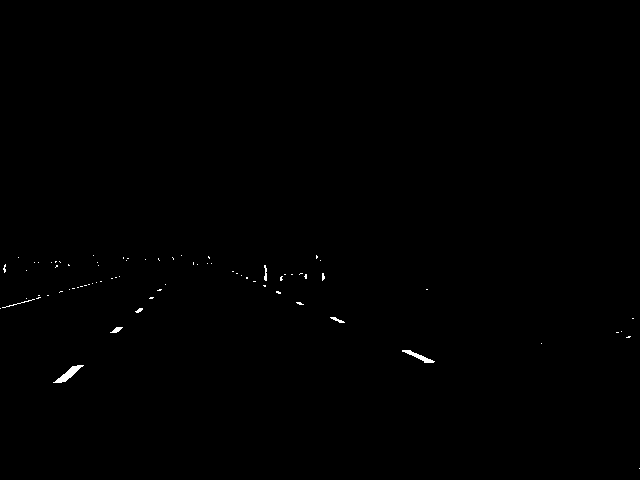
\includegraphics[width=55mm]{figures/convolution1.png} &
    \includegraphics[width=55mm]{figures/localmaxima1.png} \\
    &(a)&\\
    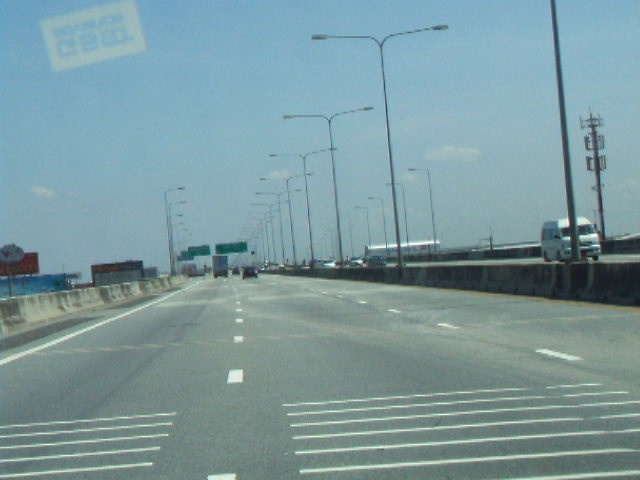
\includegraphics[width=55mm]{figures/original3.jpg} &
    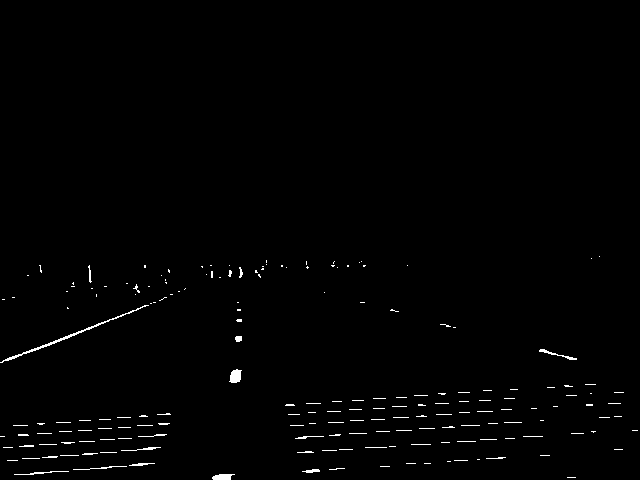
\includegraphics[width=55mm]{figures/convolution3.png} &
    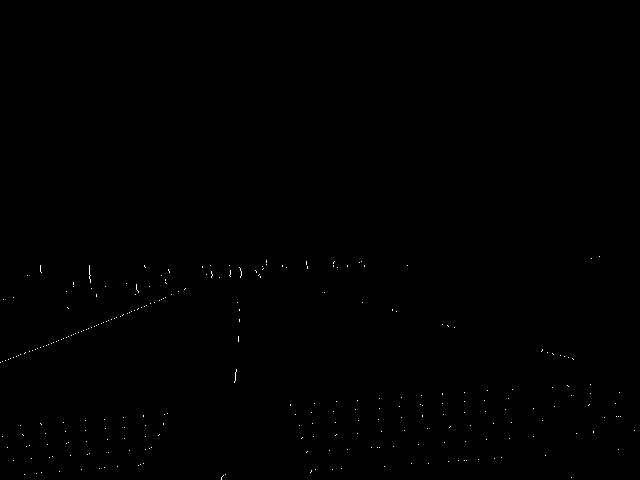
\includegraphics[width=55mm]{figures/localmaxima3.png} \\
    &(b)&\\
    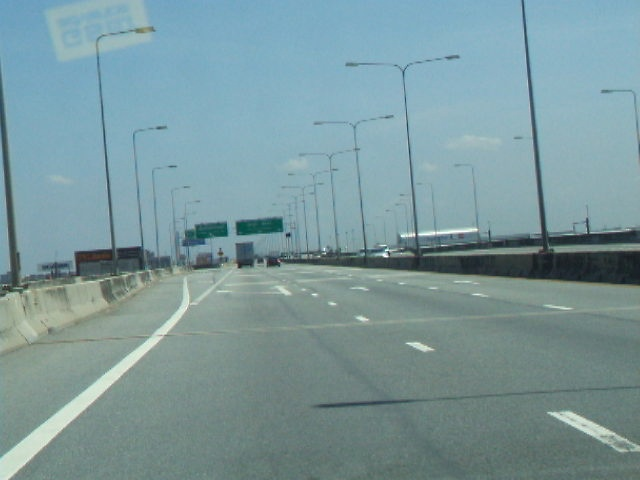
\includegraphics[width=55mm]{figures/original4.jpg} &
    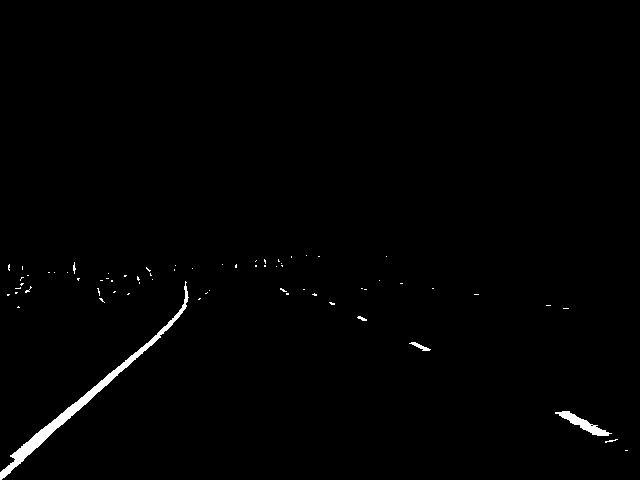
\includegraphics[width=55mm]{figures/convolution4.png} &
    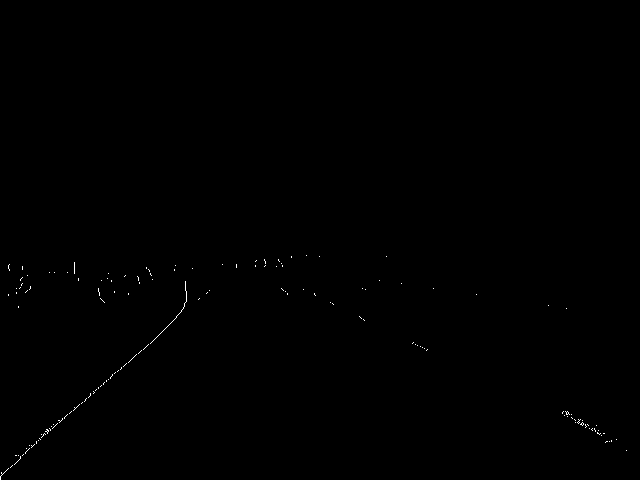
\includegraphics[width=55mm]{figures/localmaxima4.png} \\
    &(c)&\\
  \end{tabular}
  \caption{Results of matched filter convolution. Images on the left are the input image. The center and the right images are the results obtained from ``Matched Filter Convolution" and ``Non-Maximum Suppression"}
  \label{fig:matched_filter_convolution}
\end{figure}


\section{Image To Ground Plane Transformation}
Figure \ref{fig:image_to_ground_plane} shows the results of transforming points 
on the image plane to the ground plane. A major contribution to the false 
positive of the lane marking are the obstacles like vehicles in front of the 
car. If there is a vehicle in front of the camera this would result in a line 
that is almost vertical after non-maximum suppression which would result in a 
very long line when projected on the ground plane. 
\begin{figure}
  \begin{tabular}{c c c}
  \includegraphics[width=55mm]{figures/image_to_ground_plane_transformation/original1.jpg} &
    \includegraphics[width=55mm]{figures/image_to_ground_plane_transformation/localmaxima1.png} &
    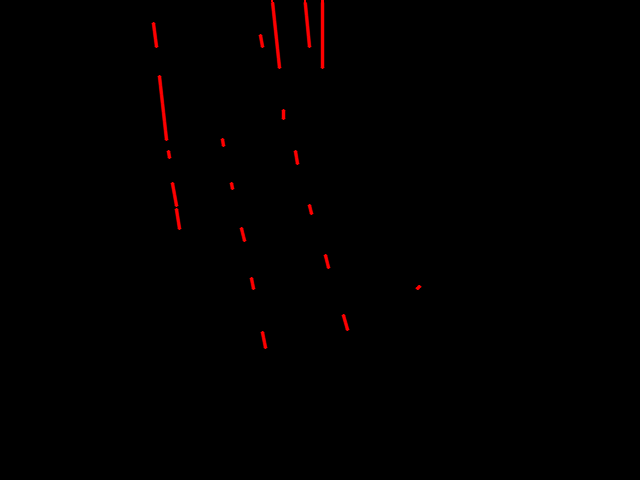
\includegraphics[width=55mm]{figures/image_to_ground_plane_transformation/ground1.png} \\
    &(a)&\\
    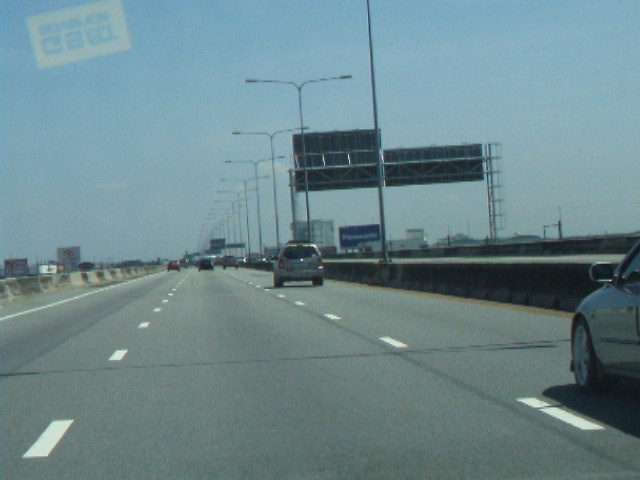
\includegraphics[width=55mm]{figures/image_to_ground_plane_transformation/original2.jpg} &
      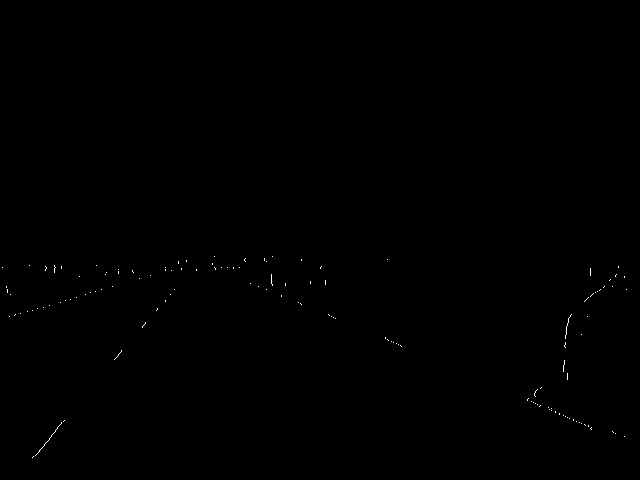
\includegraphics[width=55mm]{figures/image_to_ground_plane_transformation/localmaxima2.png} &
      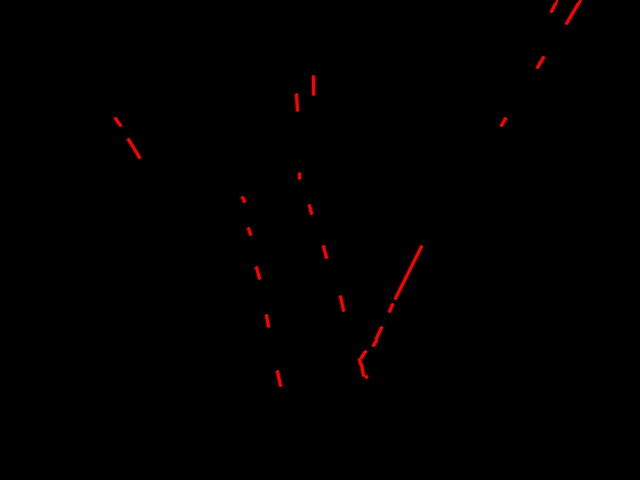
\includegraphics[width=55mm]{figures/image_to_ground_plane_transformation/ground2.png} \\
      &(b)&\\
    
  \end{tabular}
    
  \caption{Results of transforming points from image plane to ground plane. From left to right: input image, points on image plane after non-maximum suppression, results of the ground plane transformation.}
  \label{fig:image_to_ground_plane}
\end{figure}


\section{Lateral Distance of Lane Boundary}

Figure \ref{fig:lateral_distance} shows the plot of the lateral distance from 
the vehicle to the lane boundary. In red, green are the distance the left and 
right of the lane boundary. The blue line is the width of the lane. 

The figure shows the plot of 1000 frames where the car is driving straight in a 
lane. During frame 200 - 300 the cart slightly moves towards the left side of 
the lane boundary causing the change in the distance to the left and right. 

Figure \ref{fig:lane_width} plot the estimated width of the lane. Many spikes visible in the plot are due to false detection or no detection of lane marking. Causes of false detection are: 
\begin{enumerate}
  \item Shadows - Since the distance to the lane marking is calculated by picking the closest lane marking on the left and right side of the origin. Sometimes the closest lane marking on either side are not lane marking but are shadows formed when another vehicle is passing by or shadows of some other obstacles. 
  \item Speed breakers - A series of horizontal white lines which are used for slowing vehicle (Figure \ref{fig:matched_filter_convolution}) are falsely classified as lane marking and hence are also cause of incorrect distance to the lane boundary. 
\end{enumerate}

\begin{figure}
\centering
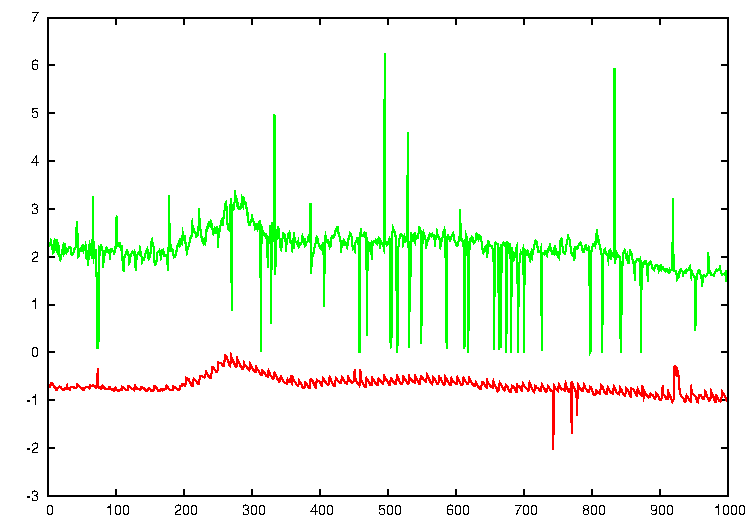
\includegraphics[width=150mm]{figures/lateral_distance.pdf}
\caption{A plot showing the lateral distance from the lane boundary. Red - distance to the left boundary, Green - distance to the right boundary}
\label{fig:lateral_distance}
\end{figure}

\begin{figure}
\centering
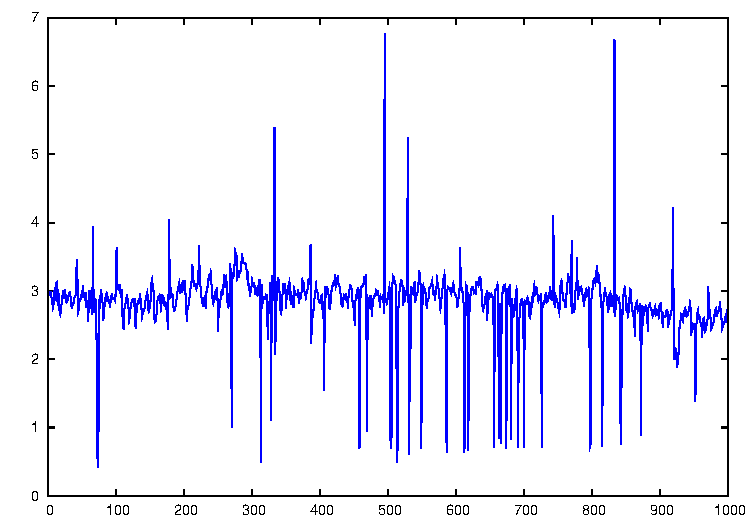
\includegraphics[width=150mm]{figures/lane_width.pdf}
\caption{A plot showing the width of the lane for 1000 frames.}
\label{fig:lane_width}
\end{figure}
